\section{Sensitivity to Deterministic Angle Variations}
\label{sec:AngleResults}

At this point in the work, it has been shown how the $\Omega$-methods
behave in problems with differing geometries and with differing materials.
However, each of these problems was run with the same deterministic calculation
parameters. While the angular flux may have differed in these problems due to
the material or geometric configuration, it did not vary due to deterministic
solver properties. This section will explore the effects of deterministic solver
choices on the $\Omega$-methods' performance.

Section \ref{sec:CharResults} showed that the $\Omega$-methods have a strong
weakness to ``thin'' materials, as CADIS and FW-CADIS do. This is because the
importance of a particle may vary several orders of magnitude over a mean free
path of travel distance. At a collision, it then requires several orders of
magnitude of sampling events. This was confirmed by
running the steel beam problem with air and concrete in place of the beam; in
the ``thin'' material air version, CADIS-$\Omega$ performs poorer than CADIS,
conversely to the original steel problem.
The characterization problem results also showed that
the incorporation of the $\Omega$-flux into a problem with materials with
strongly different moderating properties, the steel plate in concrete, showed
strong improvement when compared to both CADIS and nonbiased Monte Carlo.

Due to the better performance of CADIS-$\Omega$ than CADIS
in the problem with a steel beam in concrete, this is the problem that will be
used to characterize the $\Omega$-methods' sensitivity to deterministic angle
fidelity. In this section, the effect of deterministic solver choices on the
performance of the $\Omega$ methods will be studied. By using the same problem
with differing solver options, the effect of solver options can be isolated from
the material and geometric effects. By doing so, we seek to determine: how
resilient the $\Omega$-methods may be by using low-fidelity solver options, how
different the sensitivity of the $\Omega$-methods are to solution quality when
compared to CADIS, and how varying angular parameters may speed up or slow down
the time to a desired solution. By quantifying these effects, we can determine
the best parameter selection for the $\Omega$-methods for this type of problem
or if a desirable solution
can be sufficiently achieved using standard CADIS with a higher-quality
deterministic solution.

\subsection{Parametric Study Description}
\label{subsec:parstudy}

The angle sensitivity parametric study will cover the subset of computational parameters
that are most likely to influence the $\Omega$ method's solution. Because the
$\Omega$-flux is calculated from an angle integration of the forward and adjoint
flux, calculation parameters that are most likely to influence the angular flux
solution are the variables that were perturbed.
The two parameters that will be studied
are the quadrature order and the P$_N$ order.

The quadrature used in a deterministic solution is used do discretize the
problem in angle. Quadrature options are split into two separate selections: the
quadrature set or type, and the quadrature order. Because the $\Omega$-methods
require rotational symmetry, only quadrature sets that have rotational
symmetry (generally these are triangular quadrature sets)
can be used with the $\Omega$-methods. In ADVANTG/Denovo, the triangular
quadrature sets are: linear-discontinuous finite element, level-symmetric, and
quadruple range. As discussed previously, quadruple range is selected as the
ADVANTG default because it has good properties and guarantees positivity in the
flux. Different quadrature sets have separate
properties and are a realm of study unto their own. Thus, we will vary only
quadrature order and not quadrature type in this sensitivity study.

Quadrature orders specify
how fine of a resolution the quadrature set will be. As quadrature order
increases, the size of the angular flux matrices will increase. We expect to
observe much slower deterministic recorded times for high quadrature orders
because of the I/O demand to read and write these values. Recall that the ADVANTG
default quadrature order is 10. The quadrature orders used for the sensitivity
study aimed to choose orders surrounding this value. This resulted in quadrature
orders 5, 7, 10, 12, 15, 17, and 20 being chosen for variations in this
parameter.

The P$_N$ order determines the fidelity of the scattering expansion. The
availability of P$_N$ orders is dependent on the cross section dataset. For the
27G19N cross section library, the P$_N$ order extends to 5. As a result,
P$_N$ orders of 1, 3, and 5 are chosen for variations in this parameter.

While the P$_N$ order
does affect angular information in the problem, it will not change the size of
the angular flux matrices. As a result, deterministic runtimes between
differing P$_N$ orders
may vary, but not as significantly as they will in differing quadrature orders
due to the lack of change in I/O demands as P$_N$ order changes.

Other deterministic parameters may influence the variance reduction parameters
calculated by the $\Omega$ methods.
The spatial discretization, while not a primary factor influencing
the angular flux, still may affect the $\Omega$-methods' performance.
A finer energy group structure may also influence the $\Omega$-method solution.
Finer energy groups will more effectively reflect resonance regions in
scattering and absorption. Scattering effects in certain energy regions will
have angular dependence and, thus, may be a stronger effect on the angular flux
than a coarser energy discretization. Because these particular solution effects
are not strongly tied to influencing the angular flux, they will not be included
in the angular sensitivity parametric study. This is because the effects on the
angular flux will be hard to isolate, and conclusions drawn
from them will be harder to make. However, a study extending to include the
energy group structure, the spatial discretization, and the quadrature type
certainly could be an area of future work.

Several factors in the deterministic calculation should not have a strong effect
on the angular flux distribution. These include the spatial solver, the
convergence criteria for the solvers, and the within group solver types.
Because these factors should not influence the angular flux any more than any
other part of the solution, they will not be included in this parametric study.

\subsection{Quadrature Order}
\label{subsec:quadorder}

\begin{table}[h!]
  \centering
  \begin{tabular}{lc|ccccc}
\toprule
{} & {} & \multicolumn{2}{c}{CADIS}  & \multicolumn{2}{c}{CADIS-$\Omega$}  & analog \\
{} &  S$_N$ order &     MC  &   MC$_{hybrid}$ & MC & MC$_{hybrid}$ &  MC \\
\midrule
\multirow{7}{*}{tally avg} &  S$_N$ 5 &        683 &       677 &   1.81e+03 &
1.79e+03 &  \multirow{7}{*}{1.39} \\
      {}     &  S$_N$ 7 &   2.55e+03 &  2.53e+03 &   2.46e+03 &     2.45e+03 &    {}   \\
      {}     & S$_N$ 10 &        669 &       659 &   2.96e+03 &     2.93e+03 &    {}   \\
      {}     & S$_N$ 12 &   2.46e+03 &  2.41e+03 &        187 &          183 &    {}   \\
      {}     & S$_N$ 15 &   2.48e+03 &  2.42e+03 &   2.98e+03 &     2.92e+03 &    {}   \\
      {}     & S$_N$ 17 &   2.47e+03 &  2.39e+03 &   2.96e+03 &     2.88e+03 &    {}   \\
      {}     & S$_N$ 20 &   2.46e+03 &  2.35e+03 &   1.89e+03 &     1.81e+03 &    {}   \\
\midrule
\multirow{7}{*}{max RE}  &  S$_N$ 5 &       4.89 &      4.85 &       2.86 &
2.84 &  \multirow{7}{*}{0.0448} \\
      {}     &  S$_N$ 7 &       7.71 &      7.64 &       4.35 &         4.32 &    {}   \\
      {}     & S$_N$ 10 &       3.74 &      3.69 &       6.71 &         6.64 &    {}   \\
      {}     & S$_N$ 12 &       14.3 &      14.1 &      0.764 &        0.748 &    {}   \\
      {}     & S$_N$ 15 &       14.7 &      14.3 &       3.87 &         3.79 &    {}   \\
      {}     & S$_N$ 17 &       14.8 &      14.4 &       7.98 &         7.78 &    {}   \\
      {}     & S$_N$ 20 &       14.1 &      13.5 &       6.09 &         5.85 &    {}   \\
\midrule
\multirow{7}{*}{min RE}  &  S$_N$ 5 &   1.14e+03 &  1.13e+03 &   1.09e+03 &     1.09e+03 &      -- \\
      {}     &  S$_N$ 7 &   1.37e+03 &  1.36e+03 &   1.26e+03 &     1.25e+03 &      -- \\
      {}     & S$_N$ 10 &   1.43e+03 &  1.41e+03 &   1.32e+03 &      1.3e+03 &      -- \\
      {}     & S$_N$ 12 &   1.46e+03 &  1.43e+03 &   1.33e+03 &      1.3e+03 &      -- \\
      {}     & S$_N$ 15 &   1.47e+03 &  1.43e+03 &   1.32e+03 &      1.3e+03 &      -- \\
      {}     & S$_N$ 17 &   1.46e+03 &  1.42e+03 &   1.31e+03 &     1.28e+03 &      -- \\
      {}     & S$_N$ 20 &   1.46e+03 &  1.39e+03 &   1.31e+03 &     1.26e+03 &      -- \\
\midrule
\multirow{7}{*}{Time (mins)}  &  S$_N$ 5 &        302 &       305 &   1.13e+03 &
1.14e+03 &    \multirow{7}{*}{22.3} \\
      {}     &  S$_N$ 7 &        324 &       327 &   1.62e+03 &     1.63e+03 &    {}   \\
      {}     & S$_N$ 10 &        414 &       420 &   2.11e+03 &     2.14e+03 &    {}   \\
      {}     & S$_N$ 12 &        406 &       414 &   2.09e+03 &     2.14e+03 &    {}   \\
      {}     & S$_N$ 15 &        404 &       413 &    2.1e+03 &     2.14e+03 &    {}   \\
      {}     & S$_N$ 17 &        405 &       418 &   2.11e+03 &     2.17e+03 &    {}   \\
      {}     & S$_N$ 20 &        406 &       425 &   2.12e+03 &     2.21e+03 &    {}   \\
\bottomrule
\end{tabular}

  \caption[Figure of Merit results for steel beam embedded in concrete, with
  variations in quadrature order.]{Figure of Merit results for steel beam embedded in concrete, with
  variations in quadrature order. Subdivisions of the table indicate
calculations of the FOM using different relative errors. The analog case has a
single value for each relative error as it is not dependent on changes in
deterministic calculation parameters.}
  \label{tab:quad_foms}
\end{table}

\begin{figure}[htb!]
  \centering
  \begin{subfigure}[t]{\textwidth}
    \centering
    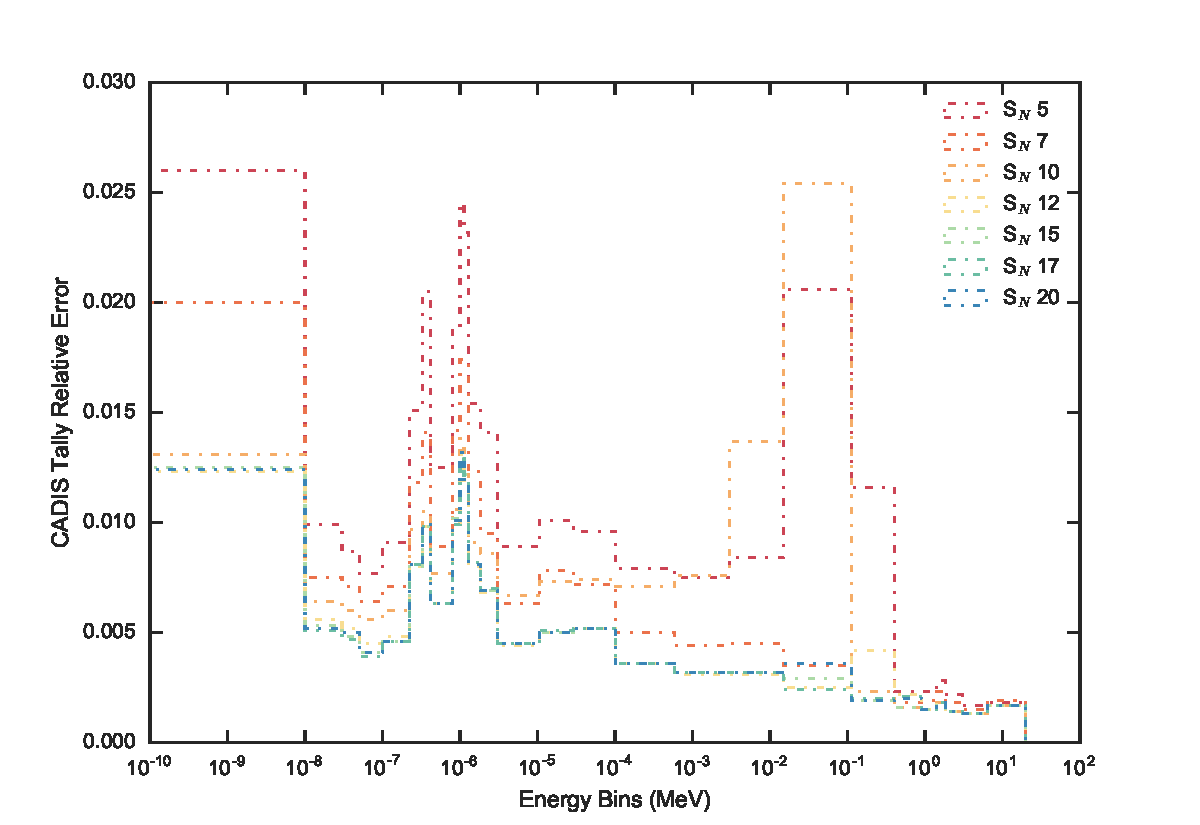
\includegraphics[width=\linewidth]{./chapters/characterization_probs/figures/angle/prob_1/err_quad_cadis.pdf}
    \caption{Relative errors of CADIS results for differing S$_N$ orders.}
    \label{fig:sn_cad_err}
  \end{subfigure}
\end{figure}
\begin{figure}[htb!]\ContinuedFloat
  \centering
  \begin{subfigure}[t]{\textwidth}
    \centering
    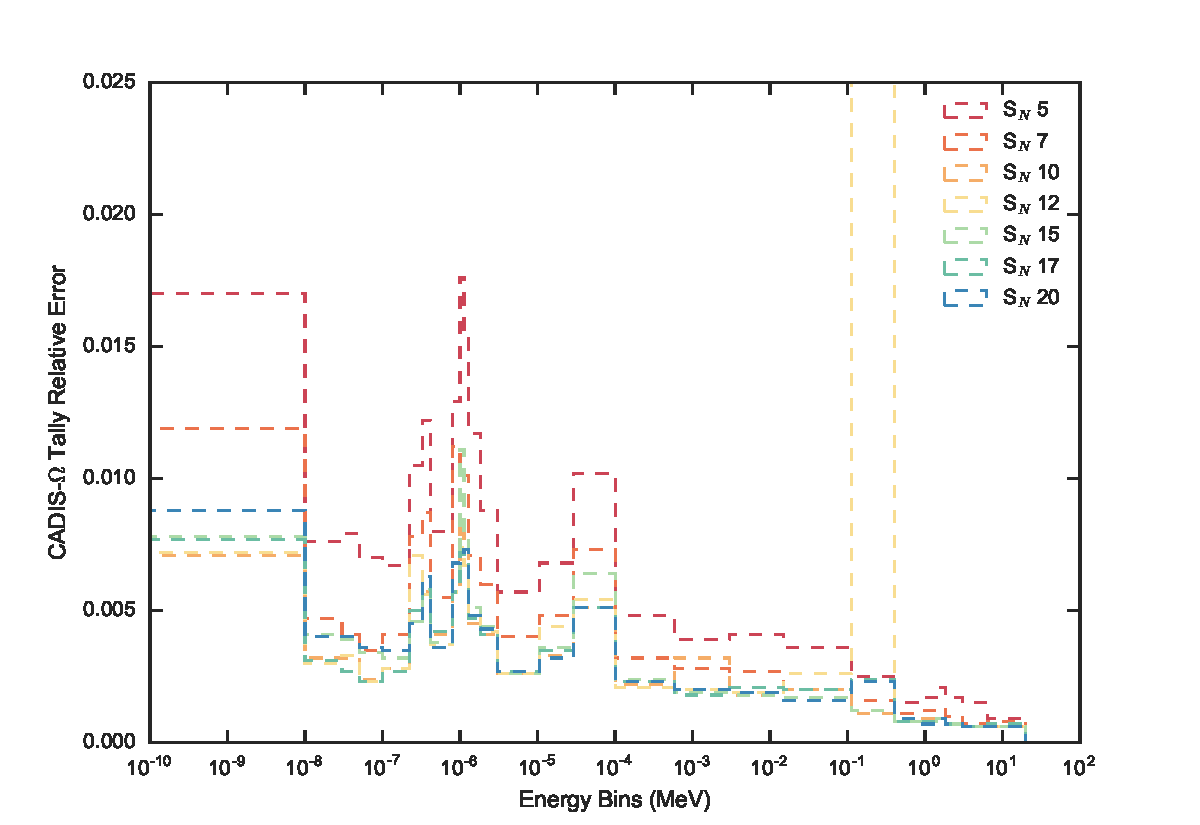
\includegraphics[width=\linewidth]{./chapters/characterization_probs/figures/angle/prob_1/err_quad_cadisangle.pdf}
    \caption{Relative errors of CADIS-$\Omega$ results for differing S$_N$
    orders.}
    \label{fig:sn_cadangle_err}
  \end{subfigure}
  \caption[Relative error results for CADIS and CADIS-$\Omega$ as a function of
  quadrature order for the problem with a steel beam in concrete.]
  {Relative error results for CADIS and CADIS-$\Omega$ as a function of
  quadrature order for the problem with a steel beam in concrete.}
\end{figure}

\begin{figure}[h!]
  \centering
  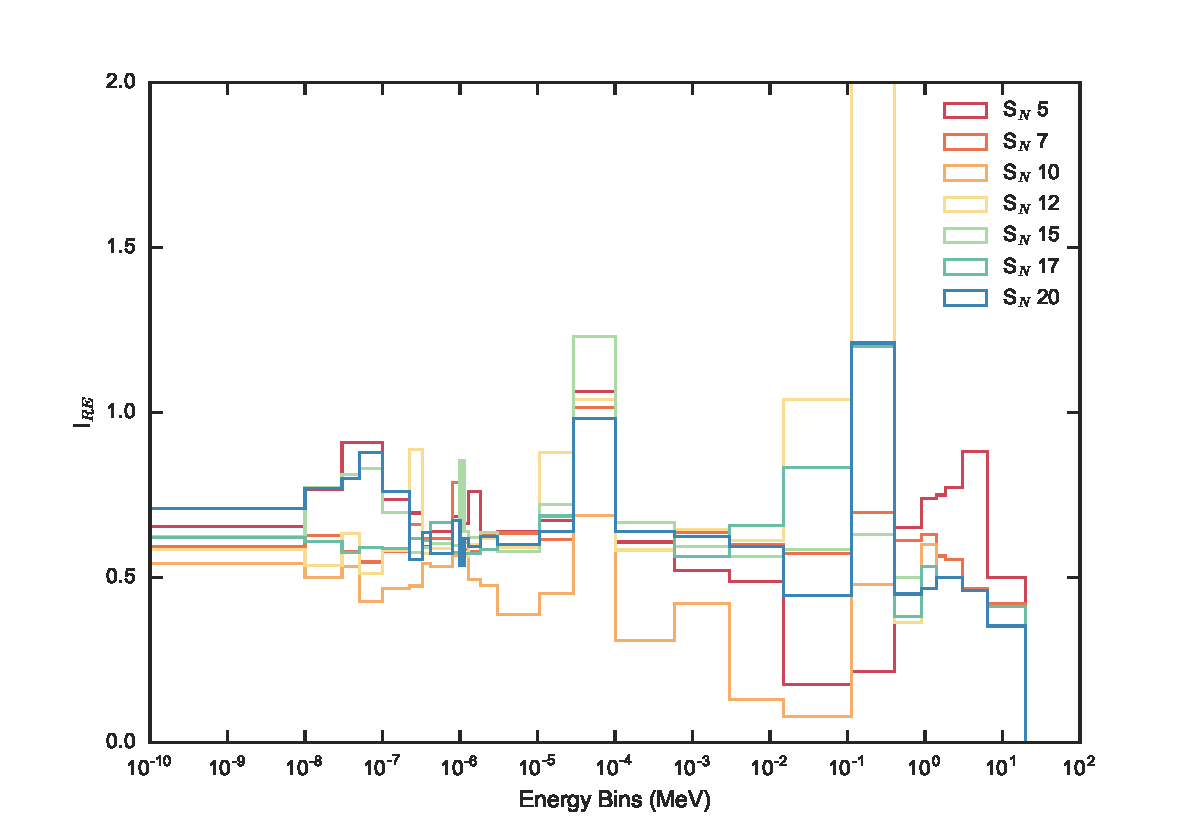
\includegraphics[height=10cm]{./chapters/characterization_probs/figures/angle/prob_1/compare_err_quad.pdf}
  \caption[Relative error improvement factor (Eq. \eqref{eq:I-RE}) between CADIS-$\Omega$ and
  CADIS as a function of quadrature order for steel beam embedded in concrete.]
  {Relative error ratio (Eq. \eqref{eq:I-RE}) between CADIS-$\Omega$ and
   CADIS as a function of quadrature order for the problem with
   a steel beam embedded in concrete.}
  \label{fig:prob_1_quad_I_RE}
\end{figure}

\begin{figure}[h!]
  \centering
  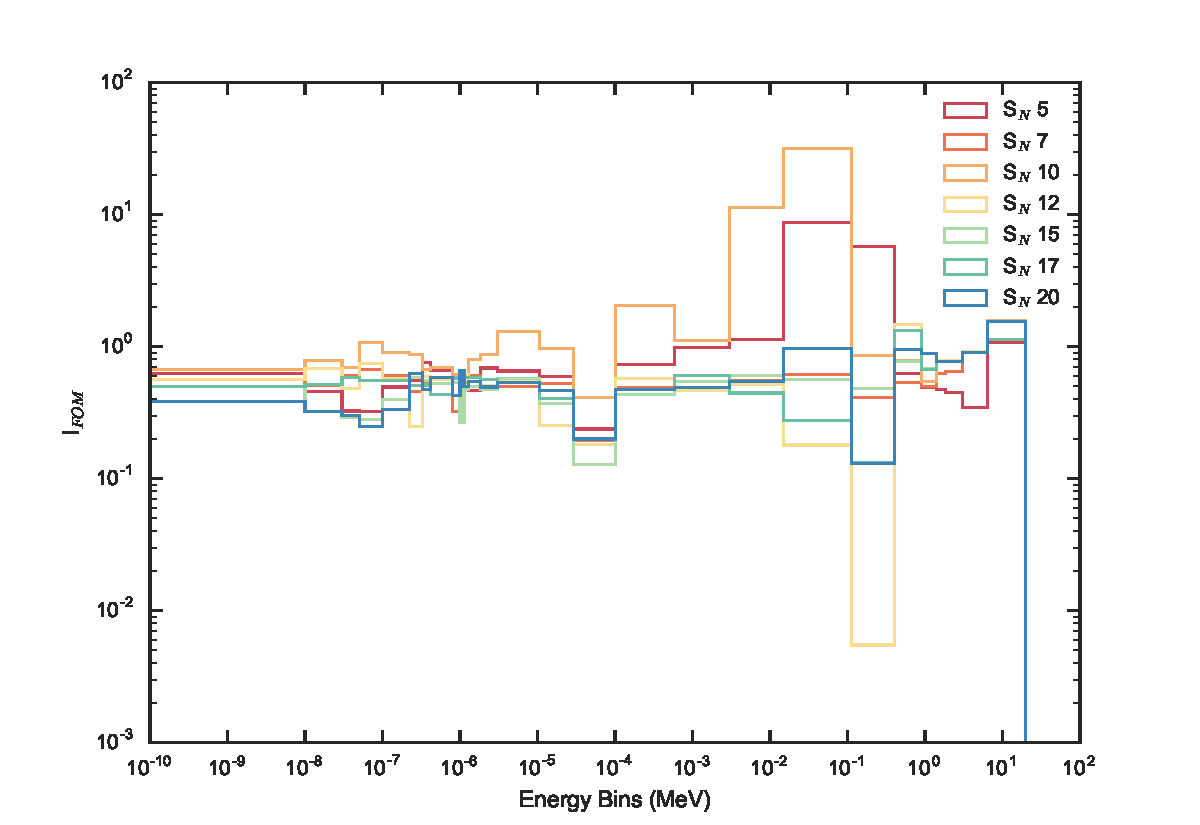
\includegraphics[height=10cm]{./chapters/characterization_probs/figures/angle/prob_1/compare_fom_quad.pdf}
  \caption[Figure of merit improvement factor  (Eq. \eqref{eq:I-FOM}) between CADIS-$\Omega$ and
  CADIS as a function of quadrature order for steel beam embedded in concrete.]
  {Figure of merit improvement factor  (Eq. \eqref{eq:I-RE}) between CADIS-$\Omega$ and
   CADIS as a function of quadrature order for the problem with
   a steel beam embedded in concrete.}
  \label{fig:prob_1_quad_I_FOM}
\end{figure}

[Show FOMs as a function of quad order for first problem] \\

[Show interesting anisotropy plots for extreme-valued quad types.] \\

[Show flux maps for each extreme-valued problem in region of interest.] \\

[Describe results.] \\

[Show FOMs as a function of quad order for second problem] \\

[Show interesting anisotropy plots for extreme-valued quad types.] \\

[Show flux maps for each extreme-valued problem in region of interest.] \\

[Describe results.] \\

\subsection{Scattering (P$_N$) Order}
\label{subsec:pnorder}

\begin{table}[h!]
  \centering
  \begin{tabular}{lc|ccccc}
\toprule
{} & {} & \multicolumn{2}{c}{CADIS}  & \multicolumn{2}{c}{CADIS-$\Omega$}  & analog \\
{} &  P$_N$ order &     MC  &   MC$_{hybrid}$ & MC & MC$_{hybrid}$ &  MC \\
\midrule
\multirow{3}{*}{tally avg} &  P$_N$ 1 &    1.76e+03 &  1.74e+03 &   2.99e+03 &
2.96e+03 &    \multirow{3}{*}{1.39} \\
     {}    &  P$_N$ 3 &         671 &       661 &   2.97e+03 &     2.94e+03 & {} \\
     {}    &  P$_N$ 5 &    2.21e+03 &  2.16e+03 &   2.45e+03 &     2.42e+03 & {}  \\
\midrule
\multirow{3}{*}{max RE} &  P$_N$ 1 &        7.19 &      7.09 &       8.06 &
7.98 &  \multirow{3}{*}{0.0448} \\
     {}    &  P$_N$ 3 &        3.75 &       3.7 &       6.74 &         6.66 & {} \\
     {}    &  P$_N$ 5 &        14.8 &      14.5 &       8.24 &         8.12 & {} \\
\midrule
\multirow{3}{*}{min RE} &  P$_N$ 1 &     1.5e+03 &  1.48e+03 &   1.33e+03 &     1.31e+03 &      -- \\
     {}    &  P$_N$ 3 &    1.43e+03 &  1.41e+03 &   1.32e+03 &     1.31e+03 &      -- \\
     {}    &  P$_N$ 5 &    1.24e+03 &  1.22e+03 &   1.57e+03 &     1.55e+03 &      -- \\
\midrule
\multirow{3}{*}{time (mins)} &  P$_N$ 1 &         394 &       399 &   2.09e+03 &
2.11e+03 &    \multirow{3}{*}{22.3} \\
     {}    &  P$_N$ 3 &         413 &       419 &    2.1e+03 &     2.13e+03 & {}  \\
     {}    &  P$_N$ 5 &         559 &       571 &   2.55e+03 &     2.59e+03 & {} \\
\bottomrule
\end{tabular}

  \caption[Figure of Merit results for steel beam embedded in concrete, with
  variations in P$_{N}$ order.]{Figure of Merit results for steel beam embedded in concrete, with
    variations in P$_{N}$ order. Subdivisions of the table indicate
calculations of the FOM using different relative errors. The analog case has a
single value for each relative error as it is not dependent on changes in
deterministic calculation parameters.}
  \label{tab:pn_foms}
\end{table}

\begin{figure}[htb!]
  \centering
  \begin{subfigure}[t]{\textwidth}
    \centering
    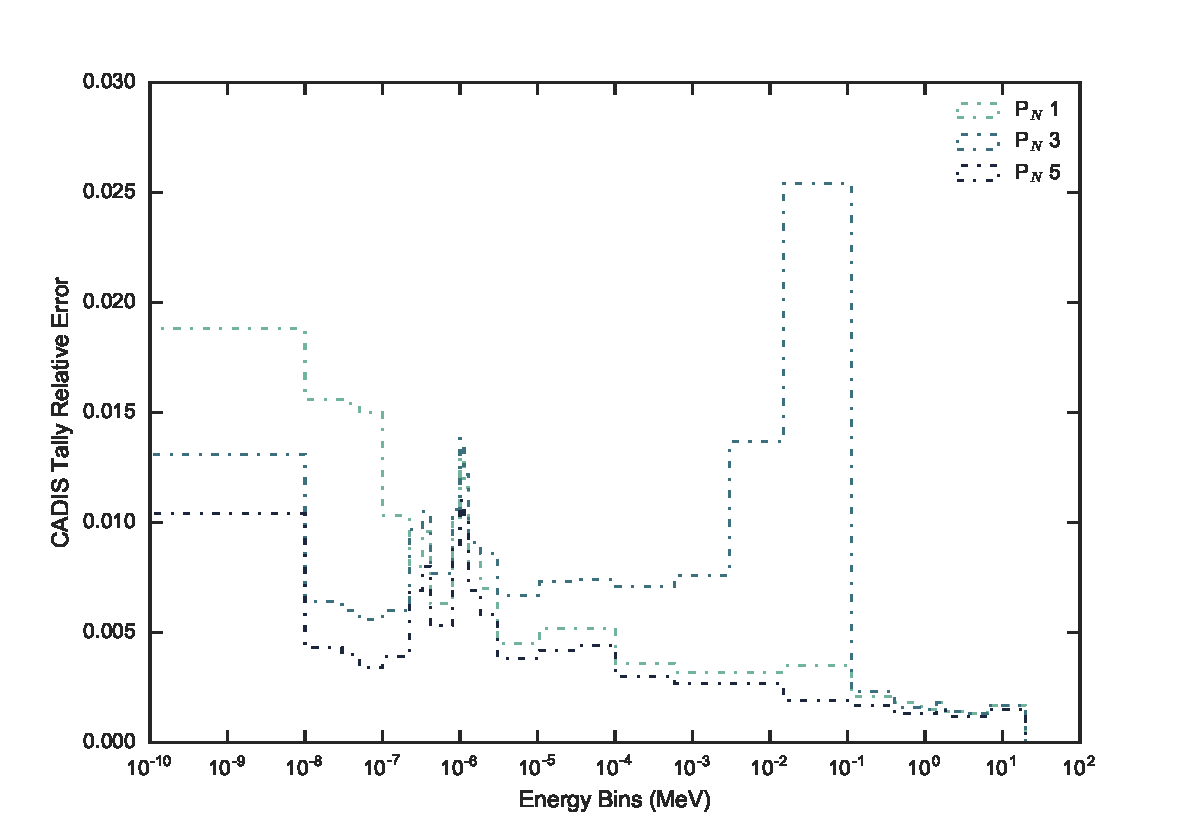
\includegraphics[width=\linewidth]{./chapters/characterization_probs/figures/angle/prob_1/err_pN_cadis.pdf}
    \caption{Relative errors of CADIS results for differing P$_N$ orders.}
    \label{fig:pn_cad_err}
  \end{subfigure}
\end{figure}
\begin{figure}[htb!]\ContinuedFloat
  \centering
  \begin{subfigure}[t]{\textwidth}
    \centering
    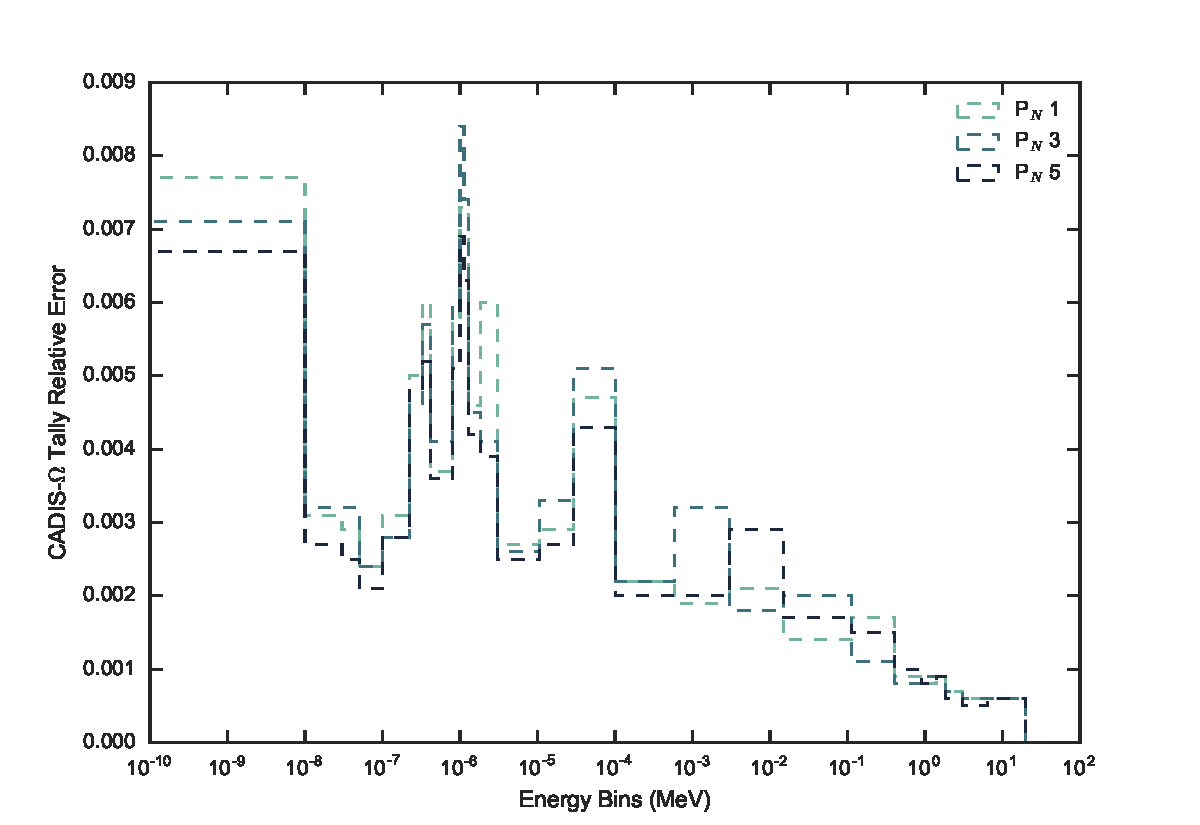
\includegraphics[width=\linewidth]{./chapters/characterization_probs/figures/angle/prob_1/err_pN_cadisangle.pdf}
    \caption{Relative errors of CADIS-$\Omega$ results for differing P$_N$
    orders.}
    \label{fig:pn_cadangle_err}
  \end{subfigure}
  \caption[Relative error results for CADIS and CADIS-$\Omega$ as a function of
  P$_N$ order for the problem with a steel beam in concrete.]
  {Relative error results for CADIS and CADIS-$\Omega$ as a function of
  P$_N$ order for the problem with a steel beam in concrete.}
\end{figure}

\begin{figure}[h!]
  \centering
  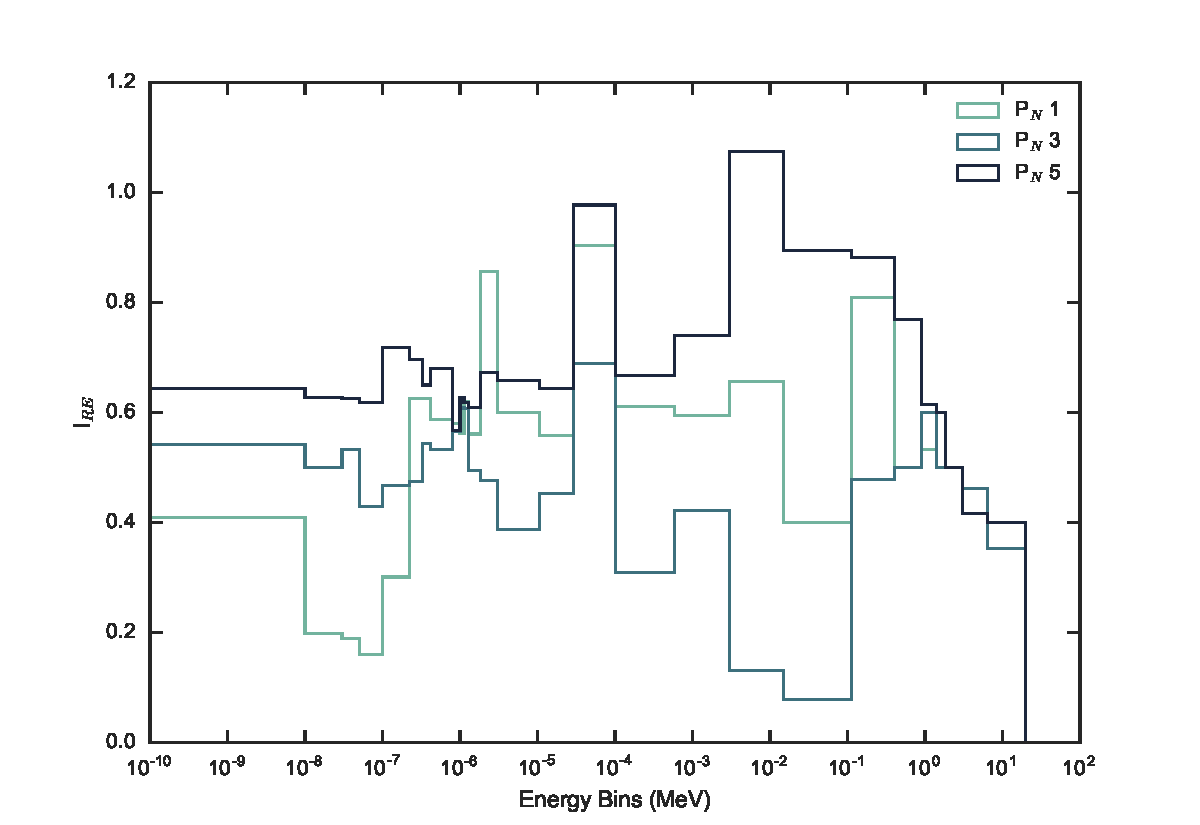
\includegraphics[height=10cm]{./chapters/characterization_probs/figures/angle/prob_1/compare_err_pN.pdf}
  \caption[Relative error improvement factor (Eq. \eqref{eq:I-RE}) between CADIS-$\Omega$ and
  CADIS as a function of P$_N$ order for steel beam embedded in concrete.]
  {Relative error improvement factor (Eq. \eqref{eq:I-RE}) between CADIS-$\Omega$ and
   CADIS as a function of P$_N$ order for the problem with a
   steel beam embedded in concrete.}
  \label{fig:prob_1_pN_I_RE}
\end{figure}

\begin{figure}[h!]
  \centering
  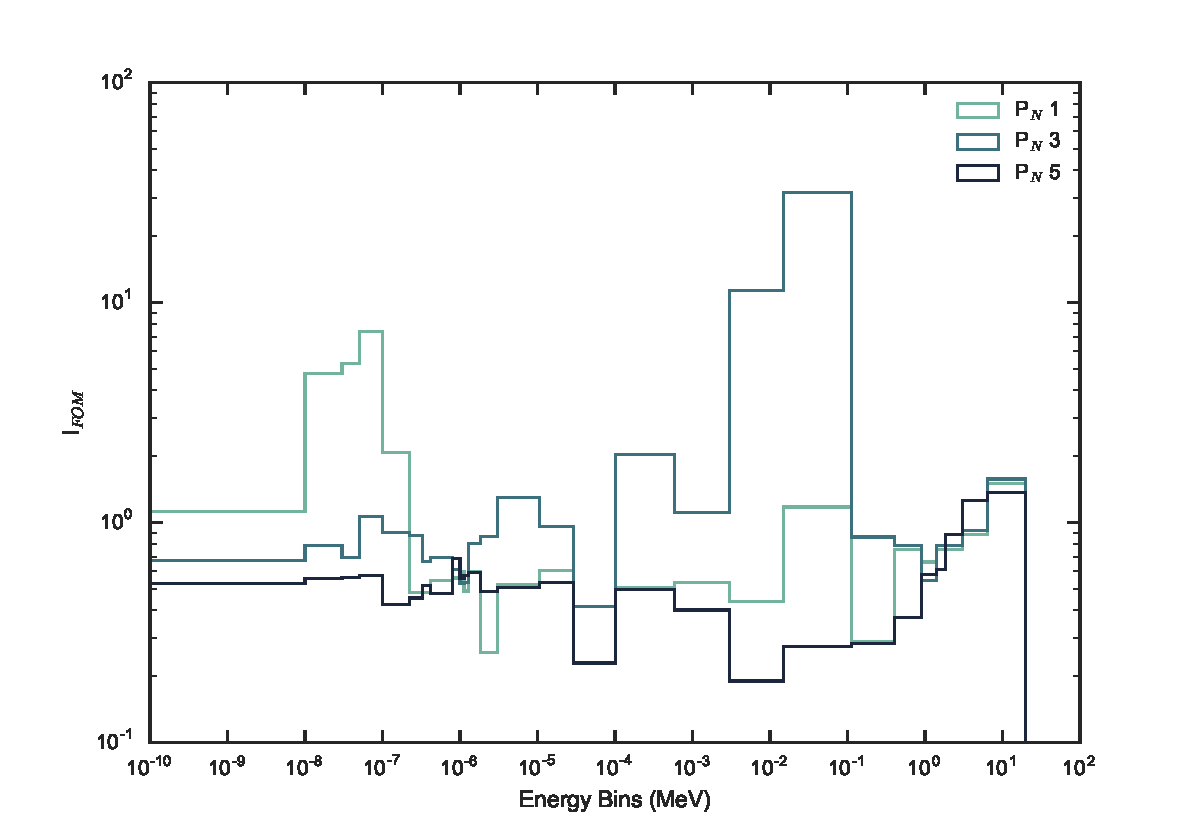
\includegraphics[height=10cm]{./chapters/characterization_probs/figures/angle/prob_1/compare_fom_pN.pdf}
  \caption[Figure of merit improvement factor (Eq. \eqref{eq:I-FOM}) between CADIS-$\Omega$ and
  CADIS as a function of P$_N$ order for steel beam embedded in concrete.]
  {Figure of merit improvement factor (Eq. \eqref{eq:I-FOM}) between CADIS-$\Omega$ and
   CADIS as a function of P$_N$ order for the problem with a
   steel beam embedded in concrete.}
  \label{fig:prob_1_pN_I_FOM}
\end{figure}

[Show FOMs as a function of pN order for first problem] \\

[Show interesting anisotropy plots for extreme-valued pN orders] \\

[Show flux maps for each extreme-valued problem in region of interest.] \\

[Describe results.] \\

[Show FOMs as a function of pN order for second problem] \\

[Show interesting anisotropy plots for extreme-valued pN orders] \\

[Show flux maps for each extreme-valued problem in region of interest.] \\

[Describe results.] \\

\subsection{Observations}
\label{subsec:observations}

\begin{figure}[h!]
  \centering
  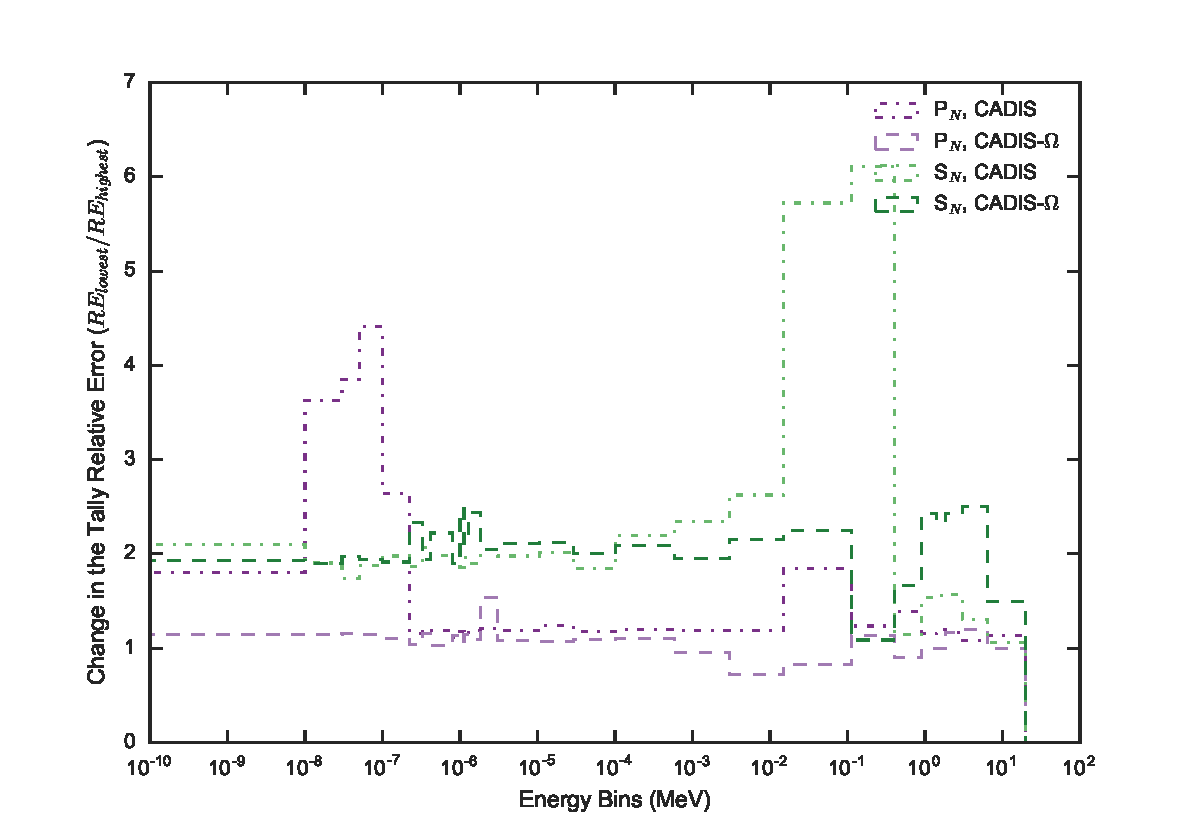
\includegraphics[height=10cm]{./chapters/characterization_probs/figures/angle/prob_1/improvement_err_allmethds.pdf}
  \caption[Ratio in the relative errors between the lowest and highest variable in the angle
  sensitivity study for CADIS and CADIS-$\Omega$.]{Ratio in the relative errors between
    the lowest and highest variable in the angle sensitivity study for CADIS and CADIS-$\Omega$.}
  \label{fig:angle_err_improvements}
\end{figure}

\begin{figure}[h!]
  \centering
  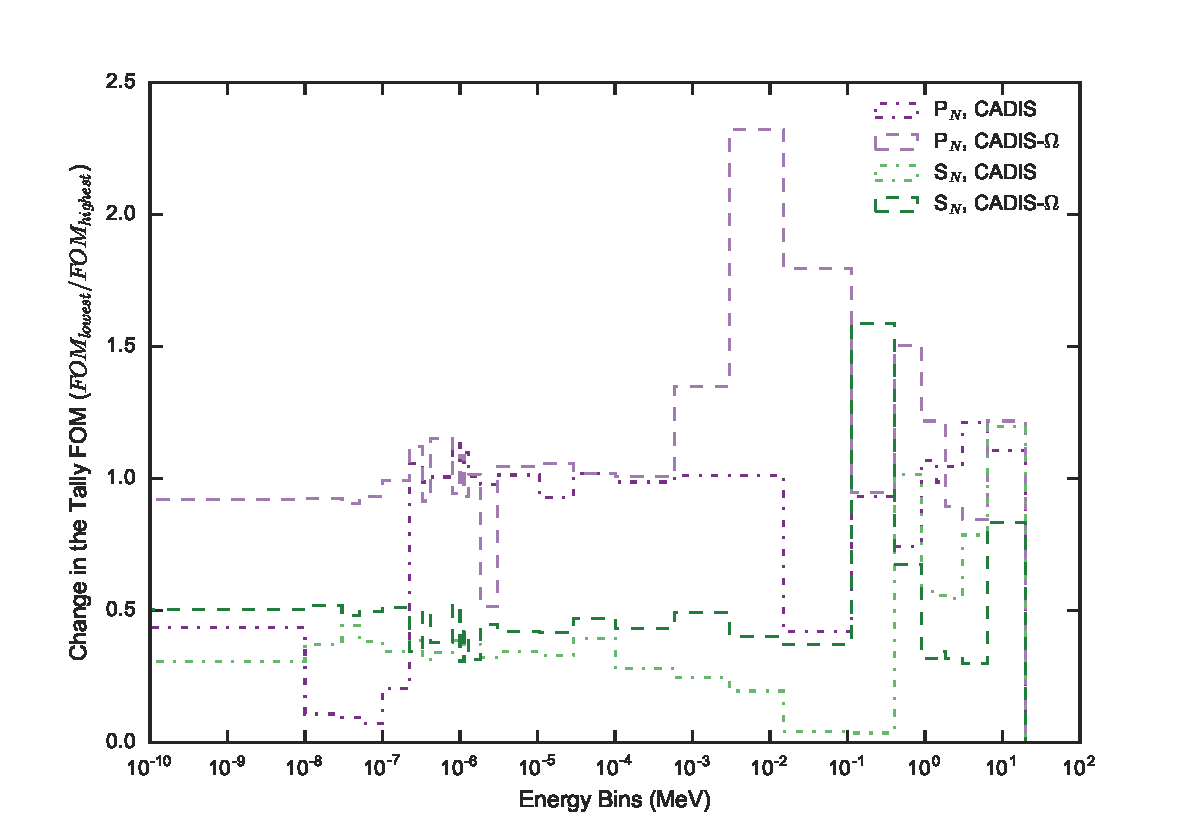
\includegraphics[height=10cm]{./chapters/characterization_probs/figures/angle/prob_1/improvement_fom_allmethds.pdf}
  \caption[Ratio in the figure of merits between the lowest and highest variable in the angle
  sensitivity study for CADIS and CADIS-$\Omega$.]{Ratio in the figure of merits between
    the lowest and highest variable in the angle sensitivity study for CADIS and CADIS-$\Omega$.}
  \label{fig:angle_fom_improvements}
\end{figure}

[Go back through results and highlight benefits and pitfalls.] \\

[Describe reasons why these might have occurred. Follow up with a list of options
that could be done in further testing to confirm reasons.] \\
